%\def\R{$\textsf{R}$}
%\def\S{$\textsf{S}$}

%\renewcommand{\labelitemii}{$\circ$}
\newcommand{\sfa}{a}
\newcommand{\worst}{\mbox{\em worst}}
\newcommand{\best}{\mbox{\em best}}
\newcommand{\regret}{\mbox{\em regret}}
\newcommand{\opt}{\mbox{\em opt}}
\newcommand{\join}{\bowtie}
\newcommand{\lE}{\underline{E}}
\newcommand{\uE}{\overline{E}}
\newcommand{\heads}{{\it heads}}
\newcommand{\tails}{{\it tails}}

\newcommand{\A}{{\cal A}}
\newcommand{\B}{{\cal B}}
\newcommand{\C}{{\cal C}}
\newcommand{\D}{{\cal D}}
\newcommand{\E}{{\cal E}}
\newcommand{\F}{{\cal F}}
\newcommand{\G}{{\cal G}}
%\newcommand{\H}{{\cal H}}
\newcommand{\I}{{\cal I}}
\newcommand{\J}{{\cal J}}
\newcommand{\K}{{\cal K}}
%\newcommand{\L}{{\cal L}}
\newcommand{\M}{{\cal M}}
\newcommand{\N}{{\cal N}}
%\newcommand{\O}{{\cal O}}
\newcommand{\Ocal}{{\cal O}}
\newcommand{\Hcal}{{\cal H}}
\renewcommand{\P}{{\cal P}}
\newcommand{\Q}{{\cal Q}}
\newcommand{\R}{{\cal R}}
%\newcommand{\S}{{\cal S}}
\newcommand{\T}{{\cal T}}
\newcommand{\U}{{\cal U}}
\newcommand{\V}{{\cal V}}
\newcommand{\W}{{\cal W}}
\newcommand{\X}{{\cal X}}
\newcommand{\Y}{{\cal Y}}
\newcommand{\Z}{{\cal Z}}


\newcommand{\IR}{\mathbb{R}}
\newcommand{\dfn}{\begin{definition}}
\newcommand{\edfn}{\end{definition}}
\newcommand{\thm}{\begin{theorem}}
\newcommand{\ethm}{\end{theorem}}
\newcommand{\xam}{\begin{example}}
\newcommand{\exam}{\end{example}}
\newcommand{\inter}{\cap}
\newcommand{\union}{\cup}




\documentclass[t, 8pt, seriff]{beamer}


%\documentclass[a4paper,xcolor=svgnames]{beamer} 
\usepackage[portuguese]{babel}
\usepackage[utf8]{inputenc}
\usepackage{times}
\usepackage{amsmath,amsthm}
\usepackage{amssymb,latexsym}
\usepackage{graphics}
%\usepackage{graphicx}

\usepackage{multimedia}
% \usepackage{movie15}
\usepackage{media9}

\usetheme{default}
%\usetheme{Singapore}
%\usetheme{PaloAlto} 
\usetheme{Boadilla}
% other themes: AnnArbor, Antibes, Bergen, Berkeley, Berlin, Boadilla, boxes, CambridgeUS, Copenhagen, Darmstadt, default, Dresden, Frankfurt, Goettingen,
% Hannover, Ilmenau, JuanLesPins, Luebeck, Madrid, Maloe, Marburg, Montpellier, PaloAlto, Pittsburg, Rochester, Singapore, Szeged, boxes, default

\useoutertheme{infolines}
%\usefonttheme{serif}
% you can also specify font themes: default, professionalfonts, serif, structurebold, structureitalicserif, structuresmallcapsserif

%\definecolor{vermelho}{RGB}{100,30,40}
%\definecolor{vermelholys}{RGB}{132,158,139}
%\definecolor{vermelholyslys}{RGB}{173,190,177}
%\definecolor{vermelholyslyslys}{RGB}{214,223,216}


%\usecolortheme[named=vermelho]{structure}




 



%\documentclass[a4paper,xcolor=svgnames]{beamer} 
%\usepackage[brazil]{babel}
%\usepackage[latin1]{inputenc}
\usepackage{ragged2e}
\usepackage{bm}
\usepackage[T1]{fontenc}
%\usepackage{amsmath,amsthm,amsfonts,amssymb} 
\usepackage{multirow}
%\usetheme{CambridgeUS} 
%\setbeamercolor{normal text}{bg=white}
\usepackage {graphicx,color}

\usepackage{wrapfig} % inserir a figura ao lado do texto
\usepackage[dvips]{epsfig} % inserir figuras de extensao post script (ps)
\usepackage{textcomp}
% \usepackage{undertilde} % colocar o til abaixo do x
\usepackage{multicol} % cor na linha
\usepackage{tabularx}
\usepackage{rotating} %rotacionar figuras e tabelas


\usepackage{ragged2e}
%\justifying


\usepackage{tikz}
\usetikzlibrary{trees}


\newtheorem{lema}{Lema}
\newtheorem{defi}{Definição}
\newtheorem{teo}{Teorema}
\newtheorem{corol}{Corolário}
\newtheorem{prop}{Proposição}


\newtheoremstyle{Exercício}{}{}{\rm}{}{\bf $\bigstar$ }{:}{ }{} %% \scshape para mudar
\theoremstyle{Exercício}
\newtheorem{exer}{Exercício}

\theoremstyle{plain}
\newtheoremstyle{Exemplo}{}{}{\rm}{}{\bf $\rhd$ }{:}{ }{} %% \scshape para mudar
%o tamanho a maiusculo
\theoremstyle{Exemplo}
\newtheorem{exem}{Exemplo}

% 
% \theoremstyle{plain}
% \newtheoremstyle{Nota}{}{}{\rm}{}{\bf\scshape}{:}{ }{}
% \theoremstyle{Nota}
 \newtheorem{nota}{Nota}






%\setlength{\rightskip}{0pt}
%\setlength{\leftskip}{0pt}
%\setlength{\spaceskip}{0pt}
%\setlength{\xspaceskip}{0pt}



\newcommand{\fullpage}[1]{
\begin{frame}
 #1
\end{frame}
}


\setbeamersize{text margin left=3em, text margin right=3em}



\setbeamertemplate{theorems}[numbered]



\definecolor{links}{HTML}{2A1B81}
\hypersetup{colorlinks,linkcolor=,urlcolor=links}


\graphicspath{{./graphics/}} 			% path das figuras (recomendável)

\newcommand{\cor}[1]{ \{{#1}\}}


\title[Probabilidade]{  Probabilidade (PPGECD000000001) \\ \vspace{1cm}Programa de Pós-Graduação em Estatística e Ciência de Dados (PGECD) }
\author[ Raydonal Ospina 
%\textcopyright 
\ ]{
	%Probabilidade\\ 
	Sessão 4 \\
	${}$ \\
	Raydonal Ospina  }

\date[]{}

\institute[UFBA]{Departamento de Estatística\\
	Universidade Federal da Bahia\\
	Salvador/BA}


\usecolortheme[rgb={0,0.6,0.6}]{structure}


%%%%%%%%%%%%%%%%%%%%%%%%%%%%%%%%%%%%%%%%%%%%%%%%%%%%%%%%%%%%%%%%%%%%%%
\begin{document}
% \SweaveOpts{concordance=TRUE}
\begin{frame}
  \titlepage
\end{frame}


\section{Probabilidade Condicional}
\begin{frame}
\frametitle{Probabilidade Condicional}

\vspace{1cm}
\begin{block}{Motivação}
	\begin{itemize}
	
\item 	A probabilidade é uma forma de quantificar a incerteza de um fenômeno. Naturalmente se obtemos mais informações sobre o fenômeno em estudo essa nova informação pode alterar,  e por vezes de forma muito significativa a avaliação da probabilidade. 
	
\item Probabilidade é baseada em informação e conhecimento. 
	
\item Nosso objetivo é saber como atualizar o valor da probabilidade quando esta base de informação ou conhecimento é alterada. Em particular, como alterar a probabilidade de um dado evento $A$ quando sabe-se que um determinado evento $B$
	ocorreu?
	\end{itemize}
\end{block}
\end{frame}

\begin{frame}{Interpretação frequentista}
	\begin{itemize}
	
	%Queremos saber qual a probabilidade de
	%um dado evento $A$, quando sabe-se que um dado evento $B$
	%ocorreu.
\item 	Seja $n$ o número de vezes que repete-se um experimento. Seja $N_A$ (resp., $N_B>0$ e
	$N_{A\cap B}$) o número de vezes que o
	evento $A$ (resp., $B$ e $A\cap B$) ocorre nessas $n$ repetições. 
	
	\item A probabilidade
	condicional  de $A$ dado que sabe-se que $B$ ocorreu, $P(A|B)$, segundo uma
	interpretação frequentista, sugere que ela deve ser igual ao limite
	das frequências relativas condicionais do evento $A$ dado o evento
	$B$, isto é, deve ser o limite $N_{A\cap B}/N_B$ quando
	$n$ tende ao infinito. Ou seja  as frequências relativas tendem a se estabilizar  ao redor de um valor específico entre 0 e 1.
	
	\item Seja $r_A=N_A/n$ a frequência relativa do
	evento $A$. 
	
	\item Note que $$\frac{N_{A\cap B}}{N_B}=\frac{r_{A\cap B}}{r_B}$$ e que segundo a interpretação
	frequentista de probabilidade $r_{A\cap B}/r_B$ é aproximadamente igual a $P(A\cap
	B)/P(B)$ para valores grandes de $n$.
	\end{itemize}
\end{frame}



\begin{frame}
\frametitle{Interpretação subjetiva}
	\begin{itemize}
\item 	Suponha que a
	incerteza de um agente é descrita por uma probabilidade $P$ em
	$(\Omega,\A)$ e que o agente observa ou fica sabendo que o evento
	$B$ ocorreu. Como o agente deve atualizar sua probabilidade
	$P(\cdot|B)$ de modo a incorporar esta nova informação? Claramente,
	se o agente $acredita$ que $B$ é verdadeiro, então parece razoável
	requerer que
	\begin{eqnarray}
	\label{eq1cond} P(B^c|B)=0.
	\end{eqnarray}
	
\item 	Em relação aos eventos contidos em $B$, é razoável assumir que sua
	chance relativa permaneça inalterada se tudo que o agente descobriu
	foi que o evento $B$ ocorreu, ou seja, se $A_1,A_2\subseteq B$ com
	$P(A_2)>0$, então
	\begin{eqnarray}
	\label{eq2} \frac{P(A_1)}{P(A_2)}=\frac{P(A_1|B)}{P(A_2|B)}.
	\end{eqnarray}
	
	Segue que (\ref{eq1cond}) e (\ref{eq2}) determinam completamente
	$P(\cdot|B)$ se $P(B)>0$.
	\end{itemize}
\end{frame}



\begin{frame}

	\begin{theorem}
		Se $P(B>0)$ e $P(\cdot|B)$ é uma medida de probabilidade em $\Omega$
		que satisfaz (\ref{eq1cond}) e (\ref{eq2}), então
		$$P(A|B)=\frac{P(A\cap B)}{P(B)}.$$
	\end{theorem}
	
	\begin{proof} Como $P(\cdot|B)$ é uma medida de probabilidade e satisfaz
	$P(B^c|B)=0$, nós temos que $P(B|B)=1-P(B^c|B)=1$. Considerando
	$A_1=A$ e $A_2=B$ em (\ref{eq2}), temos então
	$P(A|B)=\frac{P(A)}{P(B)}$ para $A\subseteq B$. Se $A$ não é um
	subconjunto de $B$, temos que $A=(A\cap B)\cup (A\cap B^c)$. Como
	$(A\cap B)$ e $(A\cap B^c)$ são eventos disjuntos, temos
	$P(A|B)=P(A\cap B|B)+P(A\cap B^c|B)$. Como $A\cap B^c\subseteq B^c$
	e $P(B^c|B)=0$, temos que $P(A\cap B^c|B)=0$. Como $A\cap B\subseteq
	B$, usando o caso anterior
	$$P(A|B)=P(A\cap B|B)=\frac{P(A\cap B)}{P(B)}.$$
	\end{proof}


Deste modo as interpretações frequentista e subjetivista da
probabilidade justificam a seguinte definição.
	
\end{frame}




\begin{frame}

	
	\begin{defi}
		Seja $(\Omega,\A,P)$ um espaço de probabilidade. Se $A,B\in \A$ e
		$P(B)>0$ a {\em probabilidade condicional de $A$ dado $B$} é
		definida por
		
		$$P(A|B)=\frac{P(A\cap B)}{P(B)}.$$
	\end{defi}


\begin{exem}
	Se atiram dois dados honestos ao ar. Qual é a probabilidade condicional de que pelo menos um resultado seja 6 dado que as faces dos dados são diferentes? Para solucionar este problema note que $\Omega =\{(a,b):a,b\in \{1,2,\ldots ,6\}\}$ e definamos os eventos 
	$$
	\begin{aligned}
	A &=\text{``Pelo menos um dado cai com a face igual a 6''} \\
	B &=\text{``As faces dos dois dados são distintas''} \\
	\end{aligned}
	$$
	Neste caso, 
	$$
	\begin{aligned}
	A = &\{(1,6),(2,6),(3,6),(4,6),(5,6),(6,1),(6,2),(6,3),(6,4), (6,5),(6,6)\}, \\ 
	B = &\{(a,b) \in \Omega\,:\,a  \neq  b\}.
	\end{aligned}
	$$
	Assim,  $$P(A|B)=\frac{P(A\cap B)}{P(B)}=\frac{\frac{10}{36}}{\frac{30}{36}}= \frac{1}{3}.$$
\end{exem}

\end{frame}

\begin{frame}
\begin{teo}[Medida de probabilidade condicional]
	Dado que $B$ ocorre, os eventos favoráveis as $A$ são aqueles que pertencem a $A\cap B.$ Assim, para $(\Omega ,{\cal F}, P)$ um espaço de probabilidade em que $B\in {\cal F}$ com $ P(B)>0$. Então:
	
	\begin{enumerate}
		\item[A.1]$P(A|B)\geq 0,$ para todo $ A\in {\cal F},$
		\item[A.2] $P(\Omega|B)=1,$ (medida finita).
		\item[A.3] ($\sigma$-aditividade) Se $A_1, A_2, \ldots$ é uma sequência de eventos de
		${\cal F}$  mutuamente excludentes, i.e., $A_i\cap A_j=\emptyset$ para todo
		$i\neq j,$ então 
		$$
		\displaystyle
		\label{ax3}
		P\left(\bigcup_{i=1}^\infty A_i \Big | B \right)=\sum_{i=1}^\infty P(A_i|B)
		$$
	\end{enumerate}
\end{teo}
	Vamos provar que para um evento fixo $B$ que satisfaz $P(B)>0$,
$P(\cdot|B)$ satisfaz os axiomas de Kolmogorov K1-K4  e realmente é uma
medida de probabilidade.
\end{frame}


\begin{frame}


\begin{proof}
 Para provar $K1$, note que para todo $A\in
	\A$, como $P(A\cap B)\geq 0$, nós temos
	$$P(A|B)=\frac{P(A\cap B)}{P(B)}\geq 0.$$
	Para provar $K2$, note que $\Omega\cap B=B$, então
	$$P(\Omega|B)=\frac{P(\Omega\cap B)}{P(B)}=\frac{P(B)}{P(B)}=1.$$
	Finalmente, para provar K4$'$ (que implica K3), note que se
	$A_1,A_2,\ldots$ são mutuamente exclusivos $A_1\cap B,A_2\cap
	B,\ldots$ também o são, então
	\begin{eqnarray}
	& & P(\cup_i A_i|B)=\frac{P((\cup_i A_i)\cap
		B)}{P(B)}=\frac{P(\cup_i(A_i\cap B))}{P(B)} \nonumber
	\\
	& & =\frac{\sum_i P(A_i\cap B)}{P(B)}=\sum_i P(A_i|B). \nonumber
	\end{eqnarray}
\end{proof}	
\end{frame}

\begin{frame}{Outras propriedades}
	\begin{enumerate}
		
		\item $P(\ \cdot \ |A)$ é uma medida de probabilidade sobre $\Omega $, que está 
		``concentrada'' em $A$, isto quer dizer, $P(A|A)=1$.
		 \item $P(A|B)=P(A\cap B|B)$;
		\item Se $A\cap B=\emptyset $, então  $P(B|A)=0.$
		
%		\item $P(B\cap C|A)=P(B|A\cap C)P(C|A)$ se $P(A \cap C)>0.$ 
		\item se $A\supseteq B$, então $P(A|B)=1$;
		\item $P(A\cap B|C)=P(A|B\cap C)P(B|C)$. 	Fazendo $C=\Omega$ na propriedade, temos que
		$P(A\inter B)=P(A|B)P(B).$
		\end{enumerate}
	

	
%Utilizando indução matemática, pode-se facilmente provar que
%\begin{eqnarray}
%& & P(A_1\inter A_2\inter \ldots \inter A_n) \nonumber \\
%& & =P(A_1)P(A_2|A_1)\ldots P(A_n|A_1\inter\ldots\inter A_{n-1}).\nonumber
%\end{eqnarray}

 \begin{teo}[Regra da multiplicação]
	Consideremos uma sequência finita de  eventos aleatórios $A_1, A_2,\ldots, A_n$ tais que os eventos condicionais $ A_i|A_1\cap A_2\cap\ldots\cap A_{i-1} $ tenham probabilidades positivas. Então temos que a probabilidade de acontecerem todos os eventos é 
	\[P\left(\bigcap_{i=1}^nA_i\right)=P(A_1)P(A_2|A_1)P(A_3|A_1\cap A_2)\ldots P(A_n|\cap_{i=1}^{n-1}A_i).\] 	
\end{teo}
\begin{proof}Use indução. Note também que \[P\left(\bigcap_{i=1}^nA_i\right)=P(A_1)\frac{P(A_1\cap A_2)}{P(A_1)}\frac{P(A_1\cap A_2\cap A_3)}{P(A_1\cap A_2)}\ldots \frac{P(\bigcap_{i=1}^n A_i)}{P(\bigcap_{i=1}^{n-1} A_i)}.\] 	
%	e usando a definição de probabilidade condicional, podemos reescrever o lado direito da igualdade acima como
%	\[P(A_1)P(A_2|A_1)P(A_3|A_1\cap A_2)\ldots P(A_n|\cap_{i=1}^{n-1}A_i)\]
%	o qual verifica a regra. 	
\end{proof}

\end{frame}

\begin{frame}
\begin{exem}
	Num jogo de cartas, três cartas, são retiradas sem substituição de um baralho (52
	cartas). Qual a probabilidade de que nenhuma das cartas retiradas seja um ouro?
	Note que qualquer carta tem a mesma probabilidade de ser retirada. Agora definamos  o evento 
	$$A_i = \{ \text{a $i$-ésima carta não é ouro}\},$$ para $i = 1, 2, 3$. Desejamos obter 
	obter $P(A_1\cap  A_2 \cap A_3)$. Lembremos que cada naipe possui 13 cartas. 
	As probabilidades condicionais deste experimento são 
	$$
	\begin{aligned}
	P(A_1) &=\frac{39}{52}, \\
	P(A_2 | A_1) &= \frac{38}{51}, \\
	P(A_3 | A_1 \cap  A_2) &= \frac{37}{50}.
	\end{aligned}
	$$
	Logo, pela regra da multiplicação
	$$P(A_1 \cap A_2 \cap A_3) =\frac{39}{52}\times\frac{38}{51}\times\frac{37}{50} \approx 0,41.$$
\end{exem}

\end{frame}

\begin{frame}
\begin{exer}	
	Um lote contém 15 moldes provenientes de um fornecedor local e 25 de um fornecedor de um estado vizinho. Três moldes são selecionados ao acaso e sem reposição. Seja $A_i$ o evento um que o $i$-ésimo molde selecionado seja proveniente do fornecedor local. Determine:
	\begin{enumerate}
		\item[(a)] $P(A_1)$.
		\item[(b)] $P(A_2|A_1)$.
		\item[(c)] $P(A_1\cap A_2)$.
		\item[(d)] $P(A_1\cup A_2)$.
		\item[(e)] $P(A_1\cap A_2\cap A_3)$.
		\item[(f)] $P(A_1\cap A_2\cap A_3^c)$.
	\end{enumerate}
\end{exer}
\end{frame}


%=====================================================================
\begin{frame}
Utilizando o seguinte teorema pode-se obter uma probabilidade (incondicional) de uma
probabilidade condicional.
\begin{teo}[Teorema da probabilidade total] 
	\label{teoBayes}
	Sejam $A_1, A_2, \ldots, A_n$ eventos dois a dois disjuntos que formam uma partição do espaço amostral, isto é, $ \displaystyle \bigcup_{i=1}^nA_i=\Omega $ e assuma que $P(A_i) > 0$  para $i = 1, 2, \ldots, n.$ Então, para qualquer evento $B$, temos que
	
	\[
	\begin{aligned}
	P(B)&=P(A_1\cap B) + \cdots + P( A_n \cap B) \\ &= P(A_1) P(B|A_1) + \cdots + P(A_n)P(B|A_n)= \displaystyle \sum_{i}P(A_i)P(B|A_i).
	\end{aligned}
	\] 	
\end{teo}
Uma representação esquemática do teorema anterior pode ser vista no gráfico da Figura \ref{fig5}.
\begin{figure}[!htb]
	\begin{center}
		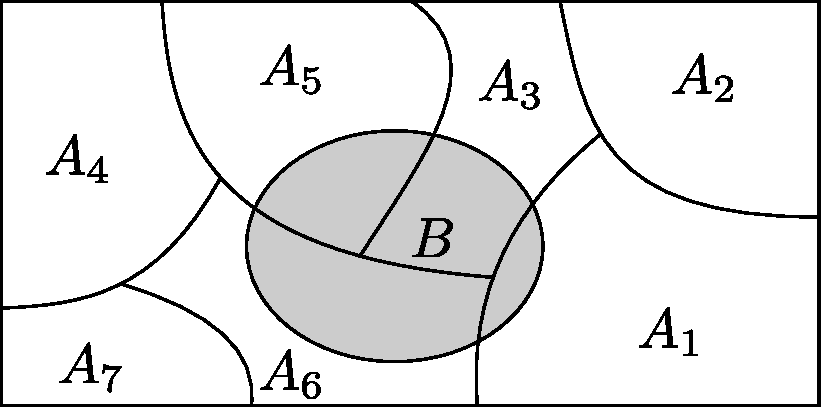
\includegraphics[angle=0, scale=0.3]{fig5.pdf}
	\end{center}
	\caption{\label{fig5} Representação esquemática do teorema da probabilidade total para $n=7$.}
\end{figure} 

\end{frame}


\begin{frame}
	\begin{proof}
		Para demonstrarmos o teorema anterior basta observarmos (ajudado pelo gráfico da Figura \ref{fig5}) que a sequência de eventos $ A_1, A_2, \ldots $ forma uma partição. Então, para qualquer $ B\subset \Omega $, segue que,  $ B=\displaystyle\bigcup_{i}(A_i\cap B) $ e como os $ A_i $ são disjuntos dois a dois temos que $ B\cap A_i $ também são disjuntos e pelo axioma K3 e pelo teorema de probabilidade total concluímos que
		$$P(B)=\displaystyle \sum_{i}P(A_i\cap B)=\sum_{i}P(A_i)P(B|A_i).$$ 	
\end{proof}
\begin{block}{Interpretação do Teorema da Probabilidade Total}
	
	$A_1,A_2,\ldots$ são possíveis
	causas e o evento $A$ é um efeito particular associado a
	uma causa, $P(B|A_i)$ especifica a relação estocástica entre a causa
	$A_i$ e o efeito $B$.
\end{block}

\end{frame}

\begin{frame}


\begin{exem}
	
	Por exemplo, seja $\{D,D^c\}$ uma partição do espaço amostral, onde $D$ é o evento que um dado indivíduo possui uma certa doença. Seja $A$ o evento que determinado teste para o diagnóstico da doença deu positivo. Então,
	\begin{itemize}
		\item $P(A|D^c)$ - {\em falso positivo}.
		\item $P(A^c|D)$ - {\em falso negativo}.
		\item Estas probabilidades determinam a qualidade do teste, quanto menores as probabilidades de falso negativo e falso positivo melhor a qualidade do teste.
	\end{itemize}
	
	Caso as probabilidades $P(D),P(A|D),P(A|D^c)$ sejam conhecidas pode-se usando o Teorema da Probabilidade Total
	obter a probabilidade incondicional de determinado exame dar positivo $P(A)$.
\end{exem}

Porém geralmente, o que se busca é saber que dado que o resultado de um exame deu positivo qual a probabilidade de
que o indivíduo esteja doente. Pode-se obter esta probabilidade utilizando a famosa {\em fórmula
	de Bayes}:
\begin{eqnarray}
& & P(D|A)=\frac{P(A\cap D)}{P(A\cap D)+P(A\cap D^c)} \nonumber \\
& & = \frac{P(A|D)P(D)}{P(A|D)P(D)+P(A|D^c)P(D^c)}. \nonumber
\end{eqnarray}
\end{frame}


\begin{frame}
Como corolário do teorema \ref{teoBayes} obtemos a muito famosa regra de Bayes, a qual constituí o alicerce da inferência Bayesiana. 

\begin{corol}[{\bf Teorema de Bayes ou regra de Bayes}] Seja $(\Omega ,{\cal F}, P)$ um espaço de probabilidade e $A_{1},A_{2},\ldots,$ uma partição 
	finita de $\Omega$, então  é satisfeita para cada
	$B\in {\cal F}$  com $P(B)>0$ a fórmula:
	$$
	P(A_{n}|B)=\frac{P(B|A_{n})P(A_{n})}{\sum_{j}P(B|A_{j})P(A_j)}, \quad \text{para todo} \quad  n.
	$$
\end{corol}

 \begin{proof}
	$$P(A_{n}|B)=\frac{P(A_{n}\cap B)}{P(B)}=
	\frac{P(B|A_{n})P(A_{n})}{\sum_{j}P(B|A_{j})P(A_{j})}.$$
\end{proof}
Para dar uma interpretação à regra de Bayes, suponhamos que os eventos $A_1, A_2, \ldots $ são todas as possíveis causas, mutuamente excludentes de um evento $B.$ Sob a suposição de que o evento $B$ tenha sido observado, a fórmula de Bayes permite conhecer qual dessas causas é a mais provável de haver produzido o evento $B.$

\end{frame}




\begin{frame}
\begin{defi}[Distribuição a priori e a posteriori]
	Seja $A_{1},A_{2},\ldots ,$ uma partição finita ou enumerável de $\Omega $, e seja $B \in {\cal F}$ com $P(B)>0$. Então 
	$P(A_{i})$ são chamadas  de probabilidades (distribuições)\textit{``a priori''}, isto é, antes de que aconteça $B.$ As probabilidades $P(A_{i}|B$ são chamadas de probabilidades (distribuições)
	\textit{``a posteriori''}, isto significa, depois que aconteceu $B.$
\end{defi}

Uma possível e muito clara regra de decisão diante uma situação de interesse, digamos a presença do evento $B$ se considere como ocorrido o evento $A_i$ como aquele que tem a maior probabilidade sob a hipótese de que o evento $B$ acontece, portanto, elege-se entre os possíveis eventos $A_i$ aquele que dando por acontecido $B$ tem a maior probabilidade de ocorrer. Naturalmente, esta decisão não está eximida de erro, mas pode ajudar a indicar a probabilidade de uma decisão falsa.

\begin{exem}
	Numa determinada cidade são feitos testes para detectar uma determinada doença. Suponhamos que  1\% das pessoas sadias são registradas como doentes,  0,1\% da população está realmente doente e  90\% dos doentes são de fato registrados como doentes. Qual é a probabilidade de que um cidadão seja registrado como doente? Qual é a probabilidade de que uma pessoa registrada como doente esteja  realmente doente?  
\end{exem}

\end{frame}

\begin{frame}

{\bf Solução:} Definamos os seguintes eventos $S$= ``sadio'', $E$= ``realmente doente'' e $T$=``registrado como doente''.  Então $P(T|\,S)=0.01$ e $P(T|\,E)=0,9$. Assim,  $$P(T)=P(T\cap (S{\huge \cup} E))=P(T|\,S)P(S)+P(T|\,E)P(E)=0,01\times 0,999+0.9\times 0,001\approx 0,01$$ e $$P(E|\,T)=P(T|\,E)P(E)/P(T)\approx 0,083.$$ Com estes resultados deduz-se  para este exemplo,  as distribuições a priori  e as distribuições a posteriori são respectivamente, (0,001, 0,999) e  (0,083, 0,917). 

\begin{exem}
	Um curso de economia possui três disciplinas de probabilidade obrigatórias (Prob I, II e III) no núcleo básico. Na primeira disciplina há 50\% dos estudantes, na segunda há 25\% dos estudantes e na terceira há 25\% dos estudantes. Todos eles pertencendo ao núcleo básico. As mulheres (M) se encontram distribuídas uniformemente, sendo que elas constituem  60\% dos alunos do núcleo básico. No gráfico da Figura \ref{arvore} estão representadas as probabilidades para este exemplo.
\end{exem}


\end{frame}

%=====================================================================
\begin{frame}



% Set the overall layout of the tree
\tikzstyle{level 1}=[level distance=3cm, sibling distance=1.5cm]
\tikzstyle{level 2}=[level distance=3cm, sibling distance=1cm]

% Define styles for bags and leafs
\tikzstyle{bag} = [circle, text width=4em, text centered]
\tikzstyle{end} = [minimum width=4pt,fill, inner sep=0pt]

\bigskip
\begin{figure}[!htbp]
	\begin{center}
		{\footnotesize
			
			% The sloped option gives rotated edge labels. Personally
			% I find sloped labels a bit difficult to read. Remove the sloped options
			% to get horizontal labels. 
			\begin{tikzpicture}[grow=right, sloped]
			
			
			\node[bag] { Cursos}
			child {
				node[bag] {Alunos}        
				child {
					node[end] {}
					edge from parent
					node[above] {M}
					node[below]  {$P(M | $Prob III $)=$ 0,6}
				}
				child {
					node[end] {}
					edge from parent
					node[above] {H}
					node[below]  {$P(H | $Prob III $)=$ 0,4}
				}
				edge from parent 
				node[above] {Prob III}
				node[below]  {$P($Prob III $)=$ 0,25}
			}
			child {
				node[bag] {Alunos}        
				child {
					node[end] {}
					edge from parent
					node[above] {M}
					node[below]  {$P(M | $Prob II $)=$ 0,6}
				}
				child {
					node[end] {}
					edge from parent
					node[above] {H}
					node[below]  {$P(H | $Prob II $)=$ 0,4}
				}
				edge from parent         
				node[above] { \ \ Prob II}
				node[below]  {$P($Prob II $)=$ 0,25}
			}
			child {
				node[bag] {Alunos}        
				child {
					node[end] {}
					edge from parent
					node[above] {M}
					node[below]  {$P(M | $Prob I $)=$ 0,6}
				}
				child {
					node[end] {}
					edge from parent
					node[above] {H}
					node[below]  {$P(H | $Prob I $)=$0,4}
				}
				edge from parent 
				node[above] {Prob I}
				node[below]  {$P($Prob I $)=$ 0,50}
			}
			%\caption{Diagrama de árvore para o exemplo das disciplinas.}
			;
			%
			\end{tikzpicture}
			\caption{\label{arvore} Diagrama de árvore para o exemplo das disciplinas de probabilidade.}
		}
	\end{center}
	
\end{figure}
\end{frame}
%=====================================================================


%\begin{frame}
%Uma forma alternativa de explorar as probabilidades, como uma medida de incerteza é através das chances (odds).
%
%\begin{defi}
%	Seja $A$ um evento aleatório,  a chance é a razão entre a probabilidade de $A$ e a probabilidade de $A^\complement$
%	$$
%	r(A) = \frac{P(A)}{1-P(A)}.
%	$$
%\end{defi}
%Consequentemente,
%$$
%P(A) = \frac{r(A)}{1+r(A)}
%$$
%Se usamos a definição clássica de probabilidade em espaços de probabilidade finitos
%$$
%P(A) =\frac{\text{``número de casos favoráveis à ocorrência do evento $A$''}}{\text{``número total de casos possíveis''}}.
%$$
%
%\begin{exem}
%	Consideremos um jogo de baralho e definamos o evento 
%	$$ A = \text{``retirar um ás de um baralho honesto de 52 cartas.''}$$
%	Claramente $P(A)=4/52$ e neste caso $r(A) = 4/48 = 1/12.$ Então dizemos que temos uma chance de 1 para doze e a denotamos por 1:12.
%\end{exem}
%
%\begin{exem}
%	Consideremos agora o exemplo do lançamento de uma moeda honesta.  Definamos o evento  
%	$$ A = \text{``a face da moeda é cara.''}$$
%	Claramente, $P(A)=1/2$ e assim $r(A)= 0.5/0.5=1.$ Assim a chance de cair uma cara é de um para um, isto é,  1:1.
%\end{exem}
%
%Podemos ainda falar em ``desvantagem'' do evento $A$ ao definir 
%$$
%\tilde{r}(A) = \frac{\text{``número de casos desfavoráveis à ocorrência do evento $A$''}}{\text{``número de casos favoráveis à ocorrência do evento $A$''}}.
%$$
%Assim a relação entre probabilidade e desvantagem é dada por
%$$
%P(A) = \frac{1}{1+\tilde{r}(A) }.
%$$
%\begin{exem}
%	Se consideramos o lançamento de um dado honesto, então $$P(\text{face ser o numero três})=1/6$$ e desta forma  a desvantagem de sair  a face com o número 3 é de  cinco para um,  isto é,  $$\tilde{r}(A) = (1-P(A))/P(A) = (5/6)/(1/6).$$
%\end{exem}
%\end{frame}

\begin{frame}
\begin{exem}
	Um fabricante produz televisores LED em três fábricas $A,$ $B$ e $C$, que respondem, respectivamente, por 40\%, 35\% e 25\% de sua produção total.
	Registros históricos da produção indicam que 2\% da produção da fábrica $A$  é defeituosa, assim como 1\% da de $B$, e 3\% da fábrica $C.$ Escolhemos um televisor aleatoriamente, e ele é defeituoso. Qual a probabilidade dele ter sido produzido na fábrica $B$?
\end{exem}	
	
	{\bf Solução:} Chamemos por $B$ o evento ``fabricado em $B$'' e ``$def$'' o evento ser defeituoso o qual pode provir de qualquer uma das 3 fábricas (e só de uma!). Logo, os eventos são mutuamente excludentes. Portanto, 
	$$
	P(def) = P(A)P(def | A)+P(B)P(def|B) + P(C)P(def|C). 
	$$
	Agora, 
	$$
	P(B|def) = \frac{(B \cap def)}{P(def)}= \frac{P(B)P(def | B)}{P(def)}
	$$
	De acordo com os dados fornecidos no problema temos
	$$
	P( def ) = ( 0,40 \times 0,02 ) + ( 0,35 \times 0,01 ) + ( 0,25 \times 0,03 ) = 0,019
	$$
	e desta forma, 
	$$
	P(B|def) = \frac{0,35 \times 0,01}{( 0,40 \times 0,02 ) + ( 0,35\times 0,01 ) + ( 0,25 \times 0,03 )}= 0,184.
	$$

\end{frame}
	
\begin{frame}
	A visualização deste problema é simplificada pela visualização do diagramas em árvore apresentado na Figura abaixo
%	\medskip
%	
	\begin{figure}[!htb]
		
		% Set the overall layout of the tree
		\tikzstyle{level 1}=[level distance=3cm, sibling distance=1.5cm]
		\tikzstyle{level 2}=[level distance=3cm, sibling distance=1cm]
		
		% Define styles for bags and leafs
		\tikzstyle{bag} = [circle, text width=4em, text centered]
		\tikzstyle{end} = [minimum width=4pt,fill, inner sep=0pt]
		\begin{center}
			{\footnotesize
				% The sloped option gives rotated edge labels. Personally
				% I find sloped labels a bit difficult to read. Remove the sloped options
				% to get horizontal labels. 
				\begin{tikzpicture}[grow=right, sloped]
				\node[bag] {Fábrica}
				child {
					node[bag] {item}        
					child {
						node[end] {}
						edge from parent
						node[above] {$a$}
						node[below]  {0,97}
					}
					child {
						node[end] {}
						edge from parent
						node[above] {$def$}
						node[below]  {0.03}
					}
					edge from parent 
					node[above] {C}
					node[below]  {0,25}
				}
				child {
					node[bag] {item}        
					child {
						node[end] {}
						edge from parent
						node[above] {$def$}
						node[below]  {0,01}
					}
					child {
						node[end] {}
						edge from parent
						node[above] {$a$}
						node[below]  {0,99}
					}
					edge from parent         
					node[above] {$B$}
					node[below]  {0,35}
				}
				child {
					node[bag] {item}        
					child {
						node[end] {}
						edge from parent
						node[above] {$def$}
						node[below]  {0,02}
					}
					child {
						node[end] {}
						edge from parent
						node[above] {$a$}
						node[below]  {0,98}
					}
					edge from parent 
					node[above] {$A$}
					node[below]  {0,40}
				};
				\end{tikzpicture}
				
				%}
			}
		\end{center}
		\caption{\label{arvore2} Diagrama de árvore para o exemplo dos televisores. As siglas $def$ indicam defeituosos e $a$ não defeituosos. }
	\end{figure}

	\begin{exem}
	Seja uma imagem com $n\times m$ pixels onde a $k$-ésima
	linha contém $d_k(\leq m)$ pixels defeituosos. Escolhe-se uma linha ao acaso e nós não sabemos qual
	foi a escolha. Em seguida, examina-se um pixel desta linha ao acaso
	e descobre-se que o pixel é defeituoso ($D$). Qual a probabilidade de que este pixel defeituoso esteja na linha $k$? \end{exem}
\end{frame}



\begin{frame}


	
	{\bf Solução:} Seja $R=k$ se o pixel pertencia a
	$k$-ésima linha da imagem. Então, sabe-se que
	$$P(R=k)=\frac{1}{n}\mbox{\ \ \ e\ \ \ }P(D|R=k)=\frac{d_k}{m}.$$
	A fórmula de Bayes nos permite determinar
	$$P(R=k|D)=\frac{\frac{1}{n}\frac{d_k}{m}}{\sum_{i=1}^{n}\frac{1}{n}\frac{d_i}{m}}=\frac{d_k}{\sum_{i=1}^{n}d_i}.$$
	
\begin{exer}
		Jogos do campeonato paulista de futebol ocorrem durante a semana e também nos fins de semana. Suponha que exatamente metade dos jogos ocorram nos fins de semana. Suponha ainda que o São Paulo ganhe 50\% dos jogos durante o fim de semana, e perca em 20\% de seus jogos no fim de semana. Finalmente, suponha que o São Paulo ganhe todos os jogos que ocorrem durante a semana.
		\begin{enumerate}
			\item[(a)] Determine a probabilidade do São Paulo empatar um jogo qualquer.
			\item[(b)] Dado que o São Paulo ganhou seu último jogo, qual a probabilidade deste jogo ter ocorrido durante a semana?
		\end{enumerate}
\end{exer}
\end{frame}


\begin{frame}
\begin{exer}
Uma urna contém 4 bolas brancas e 6 bolas pretas. Sacam-se,
sucessivamente e sem reposição, duas bolas dessa urna. Determine a
probabilidade da primeira bola ser branca sabendo que a segunda bola
é branca.
\end{exer}

{\bf Solução:} Sejam $B_1$ e $B_2$ os eventos a primeira bola é
branca e a segunda bola é branca, respectivamente. Queremos calcular
$P(B_1|B_2)$. Utilizando a fórmula de Bayes, temos
$$P(B_1|B_2)=\frac{P(B_2|B_1)P(B_1)}{P(B_2|B_1)P(B_1)+P(B_2|B_1^c)P(B_1^c)}.$$
Mas $P(B_2|B_1)=\frac{3}{9}$, $P(B_2|B_1^c)=\frac{4}{9}$,
$P(B_1)=\frac{4}{10}$ e $P(B_1^c)=\frac{6}{10}$. Logo,
$$P(B_1|B_2)=\frac{\frac{3}{9}\cdot\frac{4}{10}}{\frac{3}{9}\cdot\frac{4}{10}+\frac{4}{9}\cdot\frac{6}{10}}=\frac{\frac{2}{15}}{\frac{2}{5}}=\frac{1}{3}.$$

\begin{exer}
Uma fábrica tem 3 máquinas que produzem o mesmo ítem. As máquinas A e B são responsáveis, cada uma, por 40\% da produção. Quanto à qualidade, as máquinas A e B produzem 10\% de ítens defeituosos cada uma, enquanto a máquina C apenas 2\%. Um ítem é selecionado ao acaso da produção dessa fábrica.
\begin{enumerate}
	\item[(a)] Qual a probabilidade do ítem selecionado ser defeituoso?
	\item[(b)] Se o ítem selecionado for defeituoso, qual a probabilidade que tenha sido produzido pela máquina A?
\end{enumerate}	
\end{exer}	

\end{frame}



%%\begin{frame}
%%\begin{block}{Paradoxo de Monty Hall}
%%	Monty Hall foi um popular apresentador de programa de jogos em TV cujo jogo começava mostrando ao participante 3 portas fechadas $d_1,d_2,d_3$, e atrás de apenas uma delas havia um prêmio valioso. O participante selecionava uma porta, por exemplo, $d_1$, mas antes que a porta fosse aberta, Monty Hall, que sabia em que porta estava o prêmio, por exemplo, $d_2$, abria a porta restante $d_3$, que não continha o prêmio. O participante tinha então permissão para ficar com sua porta original, $d_1$, ou escolher a outra porta fechada. A pergunta é se é melhor ficar com a porta original ou trocar de porta.
%%\end{block}
%%
%%\begin{block}{}
%%	Vamos agora utilizar a fórmula de Bayes para analisar este problema. Seja $G$ uma porta escolhida aleatoriamente para conter o prêmio; $Y$ a porta que o participante escolhe primeiro; e $M$ a porta que Monty Hall abre. O participante não tem nenhum conhecimento a priori sobre a localização do prêmio, ou seja ele considera todas as portas equiprováveis, e isto pode ser modelado por:
%%	$$P(G=d_i|Y=d_j)=\frac{1}{3};$$
%%	todas as portas têm a mesma probabilidade de conter o prêmio não importa qual porta o participante escolhe.
%%\end{block}
%%
%%\end{frame}
%%
%%
%%\begin{frame}
%%\begin{block}{}
%%	
%%	Se o participante escolher uma porta que não contém o prêmio, Monty Hall necessariamente terá de abrir a porta que não contém o prêmio, isto pode ser modelado por:
%%	$$P(M=d_{i_1}|Y=d_{i_2},G=d_{i_3})=1,$$
%%	onde $i_1, i_2, i_3\in \{1,2,3\}$ e são distintos.
%%\end{block}
%%
%%\begin{block}{}
%%	Se o participante escolher corretamente, por exemplo, $Y=G=d_{i_2}$, então assumimos que Monty Hall escolhe aleatoriamente entre as outras duas outras portas:
%%	$$P(M=d_{i_1}|Y=G=d_{i_2})=\frac{1}{2}, \mbox{ para }d_{i_1}\ne d_{i_2}.
%%	%\footnote{A solução depende como resolvemos este caso.}
%%	$$
%%	
%%\end{block}
%%Para determinar se o participante deve trocar de porta, devemos calcular
%%\begin{eqnarray}
%%& & P(G=d_1|Y=d_2,M=d_3) \nonumber \\
%%& & =\frac{P(G=d_1,Y=d_2,M=d_3)}{P(Y=d_2,M=d_3)} \nonumber\\
%%& & =\frac{P(M=d_3|G=d_1,Y=d_2)P(G=d_1|Y=d_2)}{P(M=d_3|Y=d_2)} \nonumber \\
%%& & \times \frac{P(Y=d_2)}{P(Y=d_2)} \nonumber \\
%%%& & =\frac{P(M=d_3|G=d_1,Y=d_2)P(G=d_1|Y=d_2)}{P(M=d_3|Y=d_2)} \nonumber \\
%%& & =\frac{1/3}{P(M=d_3|Y=d_2)}. \nonumber
%%\end{eqnarray}
%%
%%\end{frame}
%%
%%
%%\begin{frame}
%%Para determinar o valor de $P(M=d_3|Y=d_2)$ utilizamos o Teorema da Probabilidade Total e a definição de probabilidade condicional:
%%\begin{eqnarray}
%%& & P(M=d_3|Y=d_2)=\frac{P(Y=d_2,M=d_3)}{P(Y=d_2)} \nonumber\\
%%& & =\frac{P(Y=d_2,M=d_3,G=d_1)}{P(Y=d_2)} + \frac{P(Y=d_2,M=d_3,G=d_2)}{P(Y=d_2)} \nonumber \\
%%& & +\frac{P(Y=d_2,M=d_3,G=d_3)}{P(Y=d_2)} \nonumber \\
%%& & =\frac{P(Y=d_2)}{P(Y=d_2)}\times [P(M=d_3|Y=d_2,G=d_1)P(G=d_1|Y=d_2)\nonumber \\
%%& & +P(M=d_3|Y=d_2,G=d_2)P(G=d_2|Y=d_2)\nonumber\\
%%& & +P(M=d_3|Y=d_2,G=d_3)P(G=d_3|Y=d_2)]\nonumber \\
%%%& & =P(M=d_3|Y=d_2,G=d_1)P(G=d_1|Y=d_2)\nonumber\\
%%%& & +P(M=d_3|Y=d_2,G=d_2)P(G=d_2|Y=d_2)\nonumber \\
%%%& & +P(M=d_3|Y=d_2,G=d_3)P(G=d_3|Y=d_2) \nonumber\\
%%& & =1\cdot \frac{1}{3}+\frac{1}{2}\cdot\frac{1}{3}+0=\frac{1}{2}.\nonumber
%%\end{eqnarray}
%%Logo, $P(G=d_1|Y=d_2,M=d_3)=\frac{2}{3}$, e o participante deve trocar de porta de sua escolha original $d_2$ para $d_1.$
%%\end{frame}
%
%
%\begin{frame}{Teorias Alternativas}
%	Embora probabilidade condicional seja bastante útil, ela sofre de
%	alguns problemas, em particular quando se quer tratar de eventos de
%	probabilidade zero. Tradicionalmente, se $P(B)=0$, então $P(A|B)$
%	não é definida. Isto leva a um número de dificuldades filosóficas em
%	relação a eventos com probabilidade zero:
%	\begin{itemize}
%		\item São eles realmente
%		impossíveis?
%		\item Caso contrário, quão improvável um evento precisa ser
%		antes de ele ser atribuído probabilidade zero?
%		\item Deve um evento em
%		algum caso ser atribuído probabilidade zero?
%		\item Se existem eventos com
%		probabilidade zero que não são realmente impossíveis, então o que
%		significa condicionar em eventos de probabilidade zero?
%	\end{itemize}
%
%\begin{exem}
%Considere o espaço de probabilidade\\ $([0,1],\B,\mu)$ onde $\B$ é a
%	$\sigma$-álgebra de Borel restrita a eventos contidos em $[0,1]$ e
%	$\mu$ é uma medida de probabilidade na qual todo intervalo em
%	$[0,1]$ possui probabilidade igual ao seu comprimento. Seja
%	$B=\{1/4,3/4\}$ e $A=\{1/4\}$. Como $\mu(B)=0$, $\mu(A|B)$ não é
%	definida. Porém parece razoável assumir que neste caso $\mu(A|B)=1/2$
%	já que $\mu$ intuitivamente implica que todos os elementos de $\Omega$ são
%	equiprováveis, mas a definição formal de probabilidade condicional
%	não nos permite obter esta conclusão.
%\end{exem}
%
%\end{frame}
%
%
%
%\begin{frame}
%
%Uma maneira de contornar alguns destes problemas é utilizar probabilidades não-padrão, que envolve conceitos de análise matemática não-padrão, que utiliza noções de infinitesimais. Outro modo é considerar probabilidades condicionais (e não
%incondicionais) como a noção fundamental. Uma medida
%de probabilidade condicional tem pares de eventos $A,B$ como
%argumentos.
%
%\begin{defi}
%Uma álgebra de Popper sobre $\Omega$ é um conjunto $\A\times \A'$ de
%subconjuntos de $\Omega\times \Omega'$ tal que (a) $\A$ é uma
%álgebra sobre $\Omega$, (b) $\A'$ é um subconjunto não-vazio de
%$\A$, e (c) $\A'$ é fechado em relação a superconjuntos em $\A$, ou
%seja, se $B\in\A'$, $B\subseteq B'$, $B'\in\A$, então $B'\in\A'$.
%\end{defi}
%
%Pode-se então definir uma medida de probabilidade condicional da
%seguinte maneira:
%\begin{defi}
%	Uma espaço de probabilidade condicional é uma tupla
%	$(\Omega,\A,\A',\mu)$ onde $\A\times \A'$ é uma álgebra de Popper
%	sobre $\Omega$ e $\mu:\A\times \A'\rightarrow [0,1]$ satisfaz:
%	\begin{enumerate}
%		\item[CP1.] $\mu(A|A)=1$ se $A\in\A'$.
%		
%		\item[CP2.] $\mu(A_1\cup A_2|B)=\mu(A_1|B)+\mu(A_2|B)$ se $A_1\cap
%		A_2=\emptyset$, $A_1,A_2\in\A$ e $B\in\A'$.
%		
%		\item[CP3.] $\mu(A_1\cap A_2|A_3)=\mu(A_1|A_2\cap A_3)\times
%		\mu(A_2|A_3)$ se $A_2\cap A_3\in \A'$ e $A_1\in\A$.
%	\end{enumerate}
%\end{defi}
%\end{frame}

\begin{frame}
	\vspace{4cm}
	\begin{block}{Independência}
		{}
	\end{block}
\end{frame}

\section{Independência}

\begin{frame}{Independência}
\begin{block}{Intuição}
	Dois eventos são independentes
	se eles não têm nada haver um com o
	outro, eles são totalmente não relacionados; a ocorrência de um não
	tem nenhuma influência sobre o outro. Por exemplo, resultados de lançamentos sucessivos de uma moeda.
\end{block}
%
\begin{defi}
	Pode-se usar probabilidades condicionais
	para formalizar esta intuição da seguinte forma, $A$ é
	independente de $B$ se $P(A|B)=P(A)$. 
	
	Mas usando a definição de
	probabilidade condicional, chega-se a seguinte conclusão $A$ é
	independente de $B$ se $P(A\cap B)=P(A)P(B)$. 
	
	Como esta última
	expressão é definida inclusive para o caso de $P(B)=0$, ela é a
	expressão adotada como a definição de independência entre eventos.
	\end{defi}

	\begin{defi}
		O evento $A$ é independente do evento $B$ se $P(A\cap B)=P(A)P(B)$.
	\end{defi}
\end{frame}
%






\begin{frame}
\begin{block}{Observações}
Note que esta definição de independência implica que independência é
um conceito simétrico em teoria da probabilidade, isto é, $A$ é
independente de $B$ se e somente se $B$ é independente de $A$. Note
que esta definição também implica que eventos $A$ e $B$ são
independentes se $P(A)=0$ ou $P(B)=0$, o que pode gerar algumas
conclusões não intuitivas se de fato $P(A)=0$ ou $P(B)=0$. Por
exemplo, se $P(A)=0$, então $A$ é independente dele mesmo, porém $A$
certamente não é não relacionado consigo mesmo.
\end{block}

\begin{teo}
	$A$ é independente dele mesmo se e somente se $P(A)=0$ ou $P(A)=1$.
\end{teo}
\begin{proof}
\begin{eqnarray}
& & P(A\cap A)=P(A)=P(A)P(A) \nonumber\\
& & \Leftrightarrow P(A)=0 \mbox{ ou } P(A)=1.\nonumber
\end{eqnarray}
\end{proof}

\end{frame}

%
\begin{frame}
\begin{exem}
	Um dado honesto é atirado ao ar duas vezes consecutivas.  Definamos os eventos $A= \ $ ``a soma dos resultados obtidos é um número par'' e $B= \ $ `` o segundo lançamento resulta ser um n\'{u}mero par''. Para este caso temos que $P(A)=P(B)=1/2$ e $P(A\cap B)=1/4$. Portanto $A$ e $B$ são eventos independentes. 
\end{exem}

\begin{exem}
	Consideremos novamente o lançamento dos dados. Mas agora carregamos o dado de tal maneira que a probabilidade de obter um n\'{u}mero par é 2/5. Se consideramos os eventos do exemplo anterior temos que $P(B)=2/5,$   $P(A)=13/25$ e $P(A\cap B)=4/25$.  Assim, $A$ e $B$ não são independentes.
\end{exem}
\end{frame}
%

\begin{frame}{Propriedades}

Intuitivamente, se $A$ é independente de $B$ o fato que $B$ não
ocorreu, ou seja que $B^c$ ocorreu, não deve alterar a probabilidade
de $A$. Portanto, é de se esperar que se $A$ e $B$ são
independentes, então $A$ e $B^c$ também são. O seguinte teorema
prova que esta intuição é verdadeira.

\begin{teo}
Se $A$ e $B$ são eventos independentes, $A$ e $B^c$ (resp., $A^c$ e
$B$, $A^c$ e $B^c$) também o são.
\end{teo}

Note que
$$A=A\cap\Omega=A\cap(B\cup B^c)=(A\cap
B)\cup(A\cap B^c).$$

Então, como $A\cap B$ e $A\cap B^c$ são mutuamente exclusivos,
axioma K3 implica que

$$P(A)=P(A\cap B)+P(A\cap B^c).$$

Como $A$ e $B$ são independentes, nós temos

$$P(A)=P(A)P(B)+P(A\cap B^c).$$

Rearranjando os termos e utilizando o fato que $P(B^c)=1-P(B)$, temos
$P(A\cap B^c)=P(A)P(B^c)$.
%\eprv


\end{frame}


\begin{frame}
\begin{proof}

%\prv
Note que
$$A=A\cap\Omega=A\cap(B\cup B^c)=(A\cap
B)\cup(A\cap B^c).$$

Então, como $A\cap B$ e $A\cap B^c$ são mutuamente exclusivos,
axioma K3 implica que

$$P(A)=P(A\cap B)+P(A\cap B^c).$$

Como $A$ e $B$ são independentes, nós temos

$$P(A)=P(A)P(B)+P(A\cap B^c).$$

Rearrajando os termos e utilizando o fato que $P(B^c)=1-P(B)$, temos
$P(A\cap B^c)=P(A)P(B^c)$.
%\eprv
\end{proof}


\end{frame}


\begin{frame}{}

\begin{block}{Coleção de Eventos}

O conceito de independência também se aplica a uma coleção
arbitrária de eventos $\{A_i\}_{i\in \I}$, onde $\I$ é um conjunto
de índices. Neste caso, têm-se duas definições.
\end{block}

\begin{defi}
	Uma coleção de eventos $\{A_i\}_{i\in \I}$ é {\em independente par a
		par} se para todo $i \ne j\in I$, $A_i$ e $A_j$ são eventos
	independentes.
\end{defi}


	\begin{defi}
		Uma sequência finita de eventos\\ $A_1,A_2,\ldots,A_n$, $n\geq 1$, é {\em
			mutuamente independente} se para todo $I\subseteq \{1,\ldots,n\}$,
		%
		$$P(\cap_{i\in I}A_i)=\prod_{i\in I}P(A_i)$$
		E uma coleção qualquer de eventos $\{A_i\}_{i\in \I}$ é mutuamente
		independente se para todo $J\subseteq \I$ finito, $\{A_i\}_{i\in J}$
		é mutuamente independente.
	\end{defi}

\end{frame}





\begin{frame}
\begin{exem}
	Consideremos os seguintes eventos relacionados com o lançamento de um dado corrente duas vezes consecutivas. Definamos os eventos  
	$A = \text{`` no primero lançamento é obtido um dois''}, $ $B =\text{`` no segundo lançamento é obtido um cinco''}$ e 
	$C =$ {`` a soma dos resultados em ambos os lançamentos é sete ''}.
	
	Neste caso, $P(A)=P(B)=P(C)=1/6$. Por outro lado, $P(A\cap B)=P(A\cap C)=P(B\cap C)=P((2,5))=1/36$. Portanto, satisfaz-se que 
	$P(A\cap B)=P(A)P(B),$ $P(A\cap C)=P(A)P(C)$ e $P(B\cap C)=P(B)P(C).$ Contudo $$P(A\cap B\cap C)=P((2,5))\neq P(A)P(B)P(C).$$
\end{exem}

\begin{exem}
Se $\Omega=\{1,2,3,4\}$ e $P(\{w\})=1/4$, então $A=\{1,2\}$,
$B=\{1,3\}$, e $C=\{2,3\}$ são eventos independentes par a par.
Pode-se verificar isto pelo fato que
$$P(A\cap B)=P(\{1\})={1}/{4}={1}/{2}\cdot{1}/{2}=P(A)P(B).$$
Similarmente, pode-se provar o mesmo resultado para os outros pares.
Contudo, a probabilidade
%
$$P(A\cap B\cap C)=P(\emptyset)=0\ne P(A)P(B)P(C)={1}/{8}.$$
Então, $A$, $B$, e $C$ não são mutuamente independentes.
\end{exem}
\end{frame}
\begin{frame}
\begin{exem}
	Certo experimento consiste em lançar um dado equilibrado duas vezes, independentemente. Dado que os dois números sejam diferentes, qual é a probabilidade condicional de
	\begin{enumerate}
		\item[(a)] pelo menos um dos números ser 6,
		\item[(b)] a soma dos números ser 8?
	\end{enumerate}
\end{exem}	
	{\bf Solução:} Para parte (a), note que existem 30 resultados possíveis para os lançamentos do dado de modo que o mesmo número não se repita, dos quais 10 o número 6 ocorre. Portanto, esta probabilidade é igual a 1/3.
	
	Para parte (b), note que existem 4 resultados possíveis que somam 8 dado que os números são diferentes, logo esta probabilidade é igual a 4/30.


\end{frame}


%\begin{frame}
%\begin{exem}
%Certo experimento consiste em lançar um dado equilibrado duas vezes, independentemente. Dado que os dois números sejam diferentes, qual é a probabilidade condicional de
%\begin{enumerate}
%\item[(a)] pelo menos um dos números ser 6,
%\item[(b)] a soma dos números ser 8?
%\end{enumerate}
%\begin{exem}
%{\bf Solução:} Para parte (a), note que existem 30 resultados possíveis para os lançamentos do dado de modo que o mesmo número não se repita, dos quais 10 o número 6 ocorre. Portanto, esta probabilidade é igual a 1/3.
%
%Para parte (b), note que existem 4 resultados possíveis que somam 8 dado que os números são diferentes, logo esta probabilidade é igual a 4/30.
%
%\end{frame}
%

\begin{frame}
\begin{exem}
Suponha que um determinado experimento é realizado repetidas vezes de forma independente e observa-se a ocorrência de determinado evento $A$ que tem probabilidade $p$. Qual é a probabilidade que $A$ ocorra $n$ vezes antes de $A^c$ ocorrer $m$ vezes?
\end{exem}

{\bf Solução:} Note que o evento $A$ ocorra $n$ vezes antes de $A^c$ ocorrer $m$ vezes é equivalente ao evento $A$ ocorrer pelo menos $n$ vezes nas primeiras $n+m-1$ repetições do experimento. Como a ordem de ocorrência do evento $A$ nas repetições não é importante e as repetiç~es são independentes, temos que o evento $A$ ocorre $k$ vezes em $n+m-1$ repetições do experimento tem probabilidade igual a:
\begin{eqnarray}
& & P(\mbox{$k$ ocorrências de $A$ em $n+m-1$ repetições}) \nonumber \\
& & =\binom{n+m-1}{k}p^k(1-p)^{n+m-1-k}. \nonumber
\end{eqnarray}
e, então,
\begin{eqnarray}
& & P(\mbox{$n$ ocorrências de $A$ antes de $m$ ocorrências de $A^c$})\nonumber \\
& & =\sum_{k=n}^{n+m-1}\binom{n+m-1}{k}p^k(1-p)^{n+m-1-k}.\nonumber
\end{eqnarray}
%\end{example}
\end{frame}


\begin{frame}

\begin{exer}
Assuma que $A_1,\ldots, A_n$ são eventos mutuamente independentes e
que $P(A_i)=p_i$. Nós calculamos as probabilidades dos seguintes
eventos:
\begin{itemize}
\item O evento $A$ é o evento que todos estes eventos ocorrem, então
%
$$P(A)=P(\cap_{i=1}^{n}A_i)=\prod_{i=1}^{n}P(A_i)=\prod_{i=1}^{n}p_i$$

\item O evento $B$ é o evento que nenhum desses eventos ocorre,
então
%
$$P(B)=P(\cap_{i=1}^{n}A_i^c)=\prod_{i=1}^{n}P(A_i^c)=\prod_{i=1}^{n}(1-p_i)$$

\item O evento $C$ é o evento que pelo menos um desses eventos ocorre,
então $C=B^c$
%
$$P(C)=P(B^c)=1-P(B)=1-\prod_{i=1}^{n}(1-p_i)$$
\end{itemize}
\end{exer}

\end{frame}


\begin{frame}
\begin{exem}
João e José disputam um jogo com uma moeda equilibrada. Cada jogador lança a moeda duas vezes e vence o jogo aquele que primeiro obtiver dois resultados iguais. João começa jogando e se não vencer passa a moeda para José e continuam alternando jogadas. Qual a probabilidade de João vencer o Jogo?
\end{exem}

{\bf Solução:} Seja $A_k$ o evento dois resultados iguais são obtidos na $k$-ésima tentativa. Note que $P(A_k)=\frac{1}{2}$. Seja $B_k$ o evento João ganha na sua $k$-ésima jogada. Então,
$$B_1=A_1;\mbox{ }B_2=A_1^c\cap A_2^c\cap A_3;\mbox{ }B_3=A_1^c\cap A_2^c\cap A_3^c\cap A_4^c\cap A_5,$$
em geral,
$$B_k=A_1^c\cap A_2^c\cap\cdots\cap A_{2k-2}^c\cap A_{2k-1}.$$
Portanto,
\begin{eqnarray}
& & P(B_k)=P(A_1^c\cap A_2^c\cap\cdots\cap A_{2k-2}^c\cap A_{2k-1}) \nonumber \\
& & =P(A_1^c)P(A_2^c)\cdots P(A_{2k-2}^c)P(A_{2k-1})=(\frac{1}{2})^{2k-1}, \nonumber
\end{eqnarray}
onde a penúltima igualdade se deve ao fato dos lançamentos serem independentes. Logo,
\begin{eqnarray}
& & P(\mbox{João vencer})=P(\cup_{k=1}^{\infty}B_k)=\sum_{k=1}^{\infty}P(B_k) \nonumber \\
& & =\sum_{k=1}^{\infty}(\frac{1}{2})^{2k-1}=\frac{2}{3}. \nonumber
\end{eqnarray}
%\end{example}
\end{frame}



\end{document}

